\documentclass[a4paper,11pt]{article}
% ---- graphiques
\usepackage{ifpdf}
\ifpdf
\usepackage[pdftex]{graphicx}
% for latex2html
\usepackage{html}
\begin{htmlonly}
\newcommand{\includecode}[2]{  \htmladdnormallink{#2}{../../#2} }
\end{htmlonly}
\else
\usepackage{graphicx}
\fi
\usepackage{wrapfig}
\usepackage{color}
%\usepackage{hyperref}



% for accents
\usepackage[latin1]{inputenc}
\usepackage[T1]{fontenc}

\usepackage{algorithm}
\usepackage{algorithmic}

\definecolor{darkgreen}{rgb}{0,0.4,0}
\definecolor{darkblue}{rgb}{0,0,0.4}
\definecolor{darkgray}{rgb}{0.2,0.2,0.2}

% ---- inclusion de codes
\usepackage{listings}
\lstset{showstringspaces=false,tabsize=4,basicstyle=\scriptsize\sffamily,breaklines=true,breakatwhitespace=true,framexleftmargin=5mm, frame=shadowbox, framesep=1pt,rulesepcolor=\color{darkgray},rulesep=.5pt,keywordstyle=\bf\color{blue},commentstyle=\color{magenta},stringstyle=\color{red},numbers=left,numberstyle=\tiny,numbersep=5pt,columns=flexible}

\lstdefinestyle{bash}{language=bash}
\lstdefinestyle{Perl}{language=Perl}
\lstdefinestyle{C++}{language=C++,emph={__global__,__shared__,__syncthreads,blockIdx,threadIdx,float3,float4},emphstyle=\bf\color{darkgreen}}
\lstdefinestyle{DTD}{language=XML}
\lstdefinestyle{XML}{language=XML,usekeywordsintag=false,markfirstintag=true}
%begin{latexonly}
\newcommand{\includecode}[2]{
\lstinputlisting[style=#1]{#2}
}
%end{latexonly}


%\lstnewenvironment{code}{}{}
\lstnewenvironment{code_bash}{\lstset{style=bash}}{}
\lstnewenvironment{code_perl}{\lstset{style=Perl}}{}
\lstnewenvironment{code_cpp}{\lstset{style=C++}}{}
\lstnewenvironment{code_dtd}{\lstset{style=DTD}}{}
\lstnewenvironment{code_xml}{\lstset{style=XML}}{}

\newcommand{\textcode}[1]{{\sf #1}}



%
\newcommand{\sofa}{SOFA}
\newcommand{\todo}[1]{}
\newcommand{\eg}{\textit{e.g.} }

\renewcommand{\vec}[1]{\ensuremath{\mathbf{#1 }}} % vector
\newcommand{\Vx}{\vec{x} } % position vector
\newcommand{\Vv}{\vec{v} } % velocity vector
\newcommand{\Va}{\vec{a} } % acceleration vector
\newcommand{\Vf}{\vec{f}} % force
\newcommand{\Vdv}{\vec{\delta\Vv}} % change of velocity vector (unknown in implicit CG, and used in constraint solver
\renewcommand{\P}{\mat{P} } % projection to a constrained space.

\newcommand{\JNL}{\mathbf{\mathcal{J}} }     % mapping des positions
\newcommand{\J}{\mat J }                 % mapping lineaire
\newcommand{\M}{\mat M }             % matrice de masse
\newcommand{\K}{\mat K }             % matrice de raideur
\newcommand{\B}{\mat B }             % matrice d'amortissement
\newcommand{\G}{\mat G }             % jacobien des contraintes



% ---- inclusion de codes
\definecolor{darkgreen}{rgb}{0,0.4,0}
\definecolor{darkblue}{rgb}{0,0,0.4}
\definecolor{darkgray}{rgb}{0.2,0.2,0.2}


% macros mathematiques
\newcommand{\ma}[1]{\ensuremath{\mathbf {#1}}}
\newcommand{\ve}[1]{\ensuremath{\mathbf {#1}}}

\usepackage{amsmath}
\usepackage{amsfonts}
\usepackage{amssymb}

% character styles
\newcommand{\bm}[1]{\ensuremath{\boldsymbol{{#1}}}}
\newcommand{\mcal}[1]{\mbox{$\mathcal #1$}} % rondes math
\newcommand{\bmcal}[1]{\mbox{\boldmath $\mathcal #1$}} % rondes grasses math
\newcommand{\ensemble}[1]{\mbox{$\mathbb{#1}$}}
\newcommand{\RRR}{\mbox{$\ensemble{R}^3$}} 


% d�finitions
\newcommand{\definition}[2]{\index{#1}{\bf #1}: #2}
\newcommand{\voc}[1]{\index{#1}#1}
\newcommand{\bvoc}[1]{\index{#1}{\bf #1}}

% misc
\newcommand{\EV}[1]{\stackrel{\rightarrow}{#1}}  % espace vectoriel
\newcommand{\EA}[1]{#1}                          % espace affine

% vectors, matrices
%\newcommand{\point}[1]{\mbox{$#1$}}          % un point
\newcommand{\point}[1]{\ensuremath{#1}}          % un point
\newcommand{\mat}[1]{\bm{#1}}         % matrice
\newcommand{\matnm}[3]{\bm{#1_{#2\times #3}}}  % matrice n lignes , m colonnes
\newcommand{\vect}[1]{\bm{#1}}        % vecteur 
%\newcommand{\vecf}[1]{\stackrel{\rightarrow}{#1}}  % vecteur avec fleche
\newcommand{\vecf}[1]{\mbox{$\overrightarrow{#1}$}}  % vecteur avec fleche
\newcommand{\ident}[1]{\bm{I_{#1}}}   % identit� en dimension n
\newcommand{\inv}[1]{#1^{-1}}         % matrice inverse
\newcommand{\psinv}[1]{#1^{+}}        % matrice pseudo-inverse
\newcommand{\transp}[1]{#1^T}         % transpos�e de 1
\newcommand{\trace}[1]{tr(#1)}        % trace
\newcommand{\deter}[1]{\mbox{$|#1|$}}       % determinant
\newcommand{\oppvec}[1]{\mbox{$\left( \vect {#1} \wedge \right)$}}  % operateur matriciel de produit vectoriel

% bases, reperes
\newcommand{\vecin}[2]{\mbox{${}^{#2}#1$}}    % vecteur 1 dans repere 2
\newcommand{\Base}[1]{\ensuremath{\mathcal B_{#1}}} % Symbole du repere 1
\newcommand{\chbase}[3]{\mbox{${}_{#2}^{#3}\mat{#1}$}}  % operateur 1 fait le passage de la base 3 vers la base 2
%\newcommand{\pchbase}[2]{\chbase{\mat{B}}{#1}{#2}}  % matrice de passage de la base 2 vers la base 1
\newcommand{\pchbase}[2]{\chbase{B}{#1}{#2}}  % matrice de passage de la base 2 vers la base 1
\newcommand{\Rep}[1]{\ensuremath{\mathcal R_{#1}}} % Symbole du repere 1
\newcommand{\rep}[1]{\Rep{#1}}                 % Symbole du repere 1
%\newcommand{\pchrep}[2]{\chbase{\mat{F}}{#1}{#2}}  % matrice de passage du repere 1 vers le repere 2, F comme Frame
\newcommand{\pchrep}[2]{\chbase{\bm{C}}{#1}{#2}}  % matrice de passage du repere 2 vers le repere 1

%% Operateur de passage du repere 1 par rapport a 2
%\newcommand{\ChgRep}[2]{\mbox{\boldmath $R_{#1}^{#2}$}}

% rotations	
%\newcommand{\rot}[2]{\mbox{$\mat{R}_{#1,#2}$}}      % rotation vectorielle
\newcommand{\rot}[2]{\ensuremath{\mat{R}_{#1,#2}}}      % rotation vectorielle
\newcommand{\rota}[3]{\mbox{$\mat{R}_{#1,#2,#3}$}}  % rotation affine

% translation
\newcommand{\trans}[2]{\mbox{$\chbase{\vect{t}}{#1}{#2}$}} % passage de #1 vers #2 par une translation, ou translation du repere #2 par rapport au repere #1

% vitesses et acc�l�rations
\newcommand{\VRep}[2]{\mbox{\boldmath $\dot R_{#1}^{#2}$}} % vitesse du repere 1 par rapport a 2 
%\newcommand{\Point}[2]{\mbox{\boldmath ${#1}^{#2}$}}  % Coordonnees d'un point 1 dans un repere 2
\newcommand{\Point}[2]{\mbox{$\vecin{\bm{#1}}{#2}$}}  % Coordonnees d'un point 1 dans un repere 2
\newcommand{\VPoint}[2]{\mbox{\boldmath ${\dot #1}_{/#2}$}} % Vitesse d'un point par rapport � un repere
\newcommand{\APoint}[2]{\mbox{\boldmath ${\ddot #1}_{/#2}$}} % Acceleration d'un point par rapport � un repere

% cinematique du solide
\newcommand{\derivedans}[2]{\mbox{$\dot{#1}^{(#2)}$}}  % derivee du vecteur 1 dans repere 2
\newcommand{\fixedans}[2]{\mbox{$#1_{\in #2}$}}        % vecteur 1 fixe dans repere 2
\newcommand{\vecom}{\mbox{$\bm{\Omega}$}}  % omega de 1 par rapport a 2
\newcommand{\vecrot}[2]{\mbox{$\vecom_{#1/#2}$}}  % omega de 1 par rapport a 2
\newcommand{\accrot}[2]{\mbox{$\dot{\vecom}_{#1/#2}$}}  % omega de 1 par rapport a 2
\newcommand{\vfdans}[3]{\mbox{$\vec V^{#2/#3}_{#1}$}}    % vitesse de 1 fixe dans 2 par rapport a 3
\newcommand{\afdans}[3]{\mbox{$\vec \Gamma^{#2/#3}_{#1}$}}    % acceleration de 1 fixe dans 2 par rapport a 3
\newcommand{\vmdans}[2]{\mbox{$\vec V^{/{#2}}_{#1}$}}    % vitesse de 1 mobile dans 2
\newcommand{\amdans}[2]{\mbox{$\vec \Gamma^{/#2}_{#1}$}}    % acceleration de 1 mobile dans 2

% chaines articulees
\newcommand{\liaison}[2]{\mbox{$\mathcal L_{#1,#2}$}}  % liaison du pere 1 vers fils 2 (et repere intermediaire)
\newcommand{\liaisonprime}[2]{\mbox{$\mathcal L'_{#1,#2}$}}  % deuxieme repere intermediaire de la liaison du pere 1 vers fils 2
\newcommand{\liaisonP}[2]{\mbox{$\mathcal L_{#1,#2}$}}  % Repere dans pere 1 de la liaison vers fils 2 
\newcommand{\liaisonC}[2]{\mbox{$\mathcal L'_{#1,#2}$}}  % Repere dans fils de la liaison du pere 1 vers fils 2 
%\newcommand{\transP}[2]{\pchrep{\liaisonP{#1}{#2}}{#1}}  % Matrice du repere dans pere de la liaison du pere 1 vers fils 2 
%\newcommand{\transC}[2]{\pchrep{\liaisonC{#1}{#2}}{#2}}  % Matrice du repere dans pere de la liaison du pere 1 vers fils 2 
%\newcommand{\transPC}[2]{\pchrep{\liaisonC{#1}{#2}}{\liaisonP{#1}{#2}}}  % matrice de passage entre repere liaison dans fils et repere de liaison dans pere
\newcommand{\transP}[2]{\chbase{C_p}{#2}{#1}}  % Matrice du repere dans pere de la liaison du pere 1 vers fils 2 
\newcommand{\transC}[2]{\chbase{C_c}{#2}{#1}}  % Matrice du repere dans pere de la liaison du pere 1 vers fils 2 
\newcommand{\transPC}[2]{\chbase{C_l}{#2}{#1}}  % matrice de passage entre repere liaison dans fils et repere de liaison dans pere
% \pchrep{fils}{pere} = \liaisonP{pere}{fils}\deplPC{pere}{fils}\liaisonC{pere}{fils}

%topology
\newcommand{\mesh}{{\mathcal M}}
\newcommand{\vertices}{{\mathcal V}}
\newcommand{\edges}{{\mathcal E}}
\newcommand{\triangles}{{\mathcal TR}}
\newcommand{\tetrahedra}{{\mathcal T}}
\newcommand{\controls}{{\mathcal C}}
\newcommand{\nvertices}{{ V}}
\newcommand{\nedges}{{ E}}
\newcommand{\ntriangles}{{ TR}}
\newcommand{\ntetrahedra}{{ TE}}
\newcommand{\ncontrols}{{C}}
\newcommand{\control}{{\mathbf C}}
\newcommand{\degree}{{d}}
\newcommand{\euc}{{\rm I\!R}}
\newcommand{\naturalSet}{{\rm I\!N}}
\newcommand{\sv}{{\mathbf D}}

\newcommand{\pctab  }{\hspace{0.15in}      }  % Pseudo-code indentation.
\newcommand{\code}[1]{ 
\begin{makeimage}
\begin{tabbing} \pctab \= \pctab \= \pctab \= \pctab \= \pctab \= \pctab \= \pctab \kill
#1
\end{tabbing}
\end{makeimage}
}
 % This file is in parent directory. Your TEXINPUTS environment variable must include .. to reach this file. Example: setenv TEXINPUTS ..:../..:${TEXINPUTS}



\graphicspath{{./}}
% ---- format de page A4
	\setlength{\textwidth }{16cm}	% largeur de ligne
	\setlength{\textheight}{23cm}   % hauteur du texte
	\setlength{\oddsidemargin}{0cm} % marge pages impaires
	\setlength{\evensidemargin}{0cm}% marge pages paires
	\setlength{\topmargin}{0cm} 	
	\setlength{\headheight}{14pt} 
	\setlength{\headsep}{0.5cm} 

%\newcommand{\trace}{{\mathrm tr}}
\newcommand{\pos}{{\mathbf X}}
\newcommand{\deformation}{{\mathbf \Phi}}
\newcommand{\strain}{{\mathbf E}}
\newcommand{\rcgd}{{\mathbf C}}
\newcommand{\spk}{{\mathbf \Sigma}}
\newcommand{\cauchy}{{\mathbf \sigma}}
\newcommand{\fpk}{{\mathbf P}}
\newcommand{\defGrad}{{\mathbf F}}
\newcommand{\identity}{\mathbf{Id}}
\newcommand{\dir}{\mathbf{e}}
\DeclareMathOperator{\Trace}{Tr}
% Title Page
\title{Pure Traction Test in Sofa}
%\author{The \sofa{} team}
\date{2014}
\author{Herv\'e Delingette\\ {\small INRIA M\'editerran\'ee, Sophia Antipolis, France}}





\begin{document} 
\maketitle

\section{Test definition}

The test consists in producing a pure strain deformation of a cylinder, {\em i.e} with 2 different stretch ratio along the $Z$ direction and the $x,y$ direction.
A pressure $p$ is applied to top disk along the main axis of the cylinder. On the bottom disk, the cylinder is free to slide such that the cylinder remains a cylinder after deformation. More precisely, in the rest configuration the height and radius of the cylinder are $h_0$ and $R_0$ whereas in the deformed configuration they are equal to $h$ and $R$ respectively.

The stretch along the main axis is written   $s_1$ such that : $h=s_1 h_0$.The stretch along the radial direction is written $s_2$ such that  $R=s_2 R_0$.

\begin{figure}[!htbp]
	\centering
    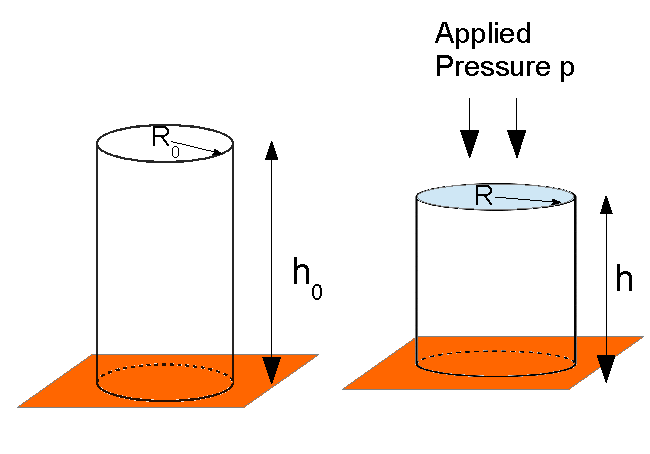
\includegraphics[width=0.80\textwidth]{PureTraction}
	\caption{Pure Traction test applied on a cylinder}
	\label{fig:PureTraction}
\end{figure}

In this case, the deformation $\deformation(\pos)$ is defined in cylindrical coordinates as $\deformation(r,\theta,z)=(s_2 r,\theta,s_1 z)$.
The deformation gradient is simply 
\begin{align*}
\defGrad &=\nabla \deformation=\left [ \begin{array}{ccc} s_2 & 0 & 0 \\0 & s_2 & 0 \\ 0 & 0 & s_1 \end{array} \right ] \\
J &= | \defGrad |= s_1 (s_2)^2 \\
\end{align*}

The right Cauchy-Green deformation tensor then writes as :
\begin{align*}
\rcgd  &=\nabla \deformation^T \nabla \deformation^T=\left [ \begin{array}{ccc} (s_2)^2 & 0 & 0 \\0 & (s_2)^2 & 0 \\ 0 & 0 & (s_1)^2 \end{array} \right ] \\
I_1 &= \Trace\rcgd=   2 (s_2)^2+  (s_1)^2  \\
I_2 &=     (s_2)^4+ 2(s_2)^2 (s_1)^2 
\end{align*}
\section{Implementation in SOFA}

A cylindrical mesh is defined with a specific engine {\em GenerateCylinder} with given number of vertices in the radial, longitudinal and circumferential directions. To have the cylinder properly deformed into a cylinder, 3 boundary conditions are combined:

\begin{itemize}
	\item Fixed node at the center of the bottom disk
	\item Nodes at the bottom disk have zero displacement along the $z$ axis
	\item One node at the bottom disk is further constrained to move along the $x$ axis. This is to avoid having the cylinder rotate along its long axis.
\end{itemize}
 
The pressure is applied on the top disk with the component {\em TrianglePressureForceField}.

\section{Mechanical Principles for Pure Traction test}

\subsection{Applied Pressure for small displacement}

Given an applied pressure $p$, and an elastic material, the objective is to compute in closed form the stretch ratio $s_1$ and $s_2$.
To this end, the total potential energy is written $W_t$ and the stretch ratios are computed as to minimize $W_t$. 

The potential energy due to the pressure force $W_e$ is given by the work of the force along the $z$ direction :
\[
W_i = -\pi (R_0)^2 ~p ~ h_0~(s_1 -1))= -V_0 p~(s_1 -1)
\]
where $V_0$ is the rest volume.

The potential energy due to the elastic material is defined as a function of strain $W_i$.

The stretch ratio $s_1$ and $s_2$ at equilibrium are obtained by solving those 2 equations :
\begin{align*}
\frac{\partial W_i}{\partial s_1} = V_0 p \\
\frac{\partial W_i}{\partial s_2} = 0 
\end{align*}

For large displacement, the force depends also on $s_2$ and therefore the force no longer derives from an energy.
However, we can still consider this potential energy as the energy of "Engineering pressure" and compute equilibrium position for it.

\subsection{Stress Analysis}

In large displacement, it is sufficient to consider :

\begin{itemize}
	\item the divergence of the first Piola-Kirchoff stress tensor should be 0
	\item the Cauchy stress as boundary conditions.
\end{itemize}

The second Piola-Kirchoff stress tensor is defined based on the derivative of the strain function : $\spk=\frac{\partial W}{\partial \strain}$.
We have $E_{11}=E_{22}=\frac{(s_2)^2-1}{2}$ and $E_{33}=\frac{(s_1)^2-1}{2}$.

Thus the second Piola-Kirchoff stress tensor correspond to derivatives of the energy with respect to $(s_1)^2$ and  $(s_2)^2$ : $\spk_{11}=2\frac{\partial W}{\partial (s_2)^2}$ $\spk_{33}=2\frac{\partial W}{\partial (s_1)^2}$ 

The first Piola-Kirchoff $\fpk=\defGrad \spk$ is independent of the point in space and therefore its divergence is null which satisfies the equation of motion in absence of any applied volumetric force. 

The Cauchy stress $\cauchy=\frac{1}{J} \defGrad \spk \defGrad^T$ is the state of stress in the deformed configuration. Clear at equilibrium, one should have $\cauchy_{11}=\cauchy_{22}=0$ and $\cauchy_{33}=p$. The first equation boils down to $\frac{\partial W}{\partial (s_2)^2}=0$ while the second leads to $\frac{\partial W}{\partial (s_1)^2}=\frac{p (s_2)^2}{2 s_1}$. The latter may also be written as $\frac{\partial W}{\partial s_1}=\frac{\partial W}{\partial (s_1)^2} \frac{\partial (s_1)^2}{\partial s_1}= p (s_2)^2$

A more general formula exists providing the expression of the Cauchy stress 

\subsection{Energy Analysis}
The total energy of the cylinder is given by the sum of the strain energy and the pressure energy. The equilibrium position is found as the position parameterized by $s_1$ and $s_2$ which minimizes the sum of the energies.

The ene

\section{Pure Traction test for a linear elastic material}

The linearized strain $\strain_L= \frac{1}{2}(\defGrad + \defGrad^T -2\identity)$ is then :
\begin{align*}
\strain_L  &=  \left [ \begin{array}{ccc} s_2-1 & 0 & 0 \\0 & s_2-1 & 0 \\ 0 & 0 & s_1-1 \end{array} \right ] =  \left [ \begin{array}{ccc} e_2 & 0 & 0 \\0 & e_2 & 0 \\ 0 & 0 & e_1 \end{array} \right ]
\end{align*}

The strain energy is then given as :
\begin{align*}
W_i^{L}&=V_0 (\frac{\lambda}{2}  (\trace \strain_L)^2 + \mu \trace \strain^2) \\
&=V_0 (\frac{\lambda}{2}  (e_1+2 e_2)^2 +\mu ((e_1)^2+2 (e_2)^2)) 
\end{align*}

From $\frac{\partial W_i}{\partial s_2} = \frac{\partial W_i}{\partial e_2}\frac{\partial e_2}{\partial s_2}= 0$ we obtain that the radial stretch $s_2$ is proportional to the longitudinal stretch $s_1$ :
\[
e_2 = \frac{-\lambda}{2(\lambda+\mu)} e_1 = -\nu e_1
\] where $\nu$ is the Poisson coefficient.
From $\frac{\partial W_i}{\partial s_1} = \frac{\partial W_i}{\partial e_1}\frac{\partial e_1}{\partial s_1}= V_0 p$ we obtain that the longitudinal stretch $s_1$ is proportional to the applied pressure $p$ :
\[
e_1 = \frac{\lambda+\mu}{\mu(3\lambda+2\mu)} p = \frac{p}{E} 
\] where $E$ is the Young Modulus.

For $E=1$ and $\nu=0.45$ the following curves are obtained for $s_1$ (red) and $s_2$ (blue).
\begin{figure}[!htbp]
	\centering
    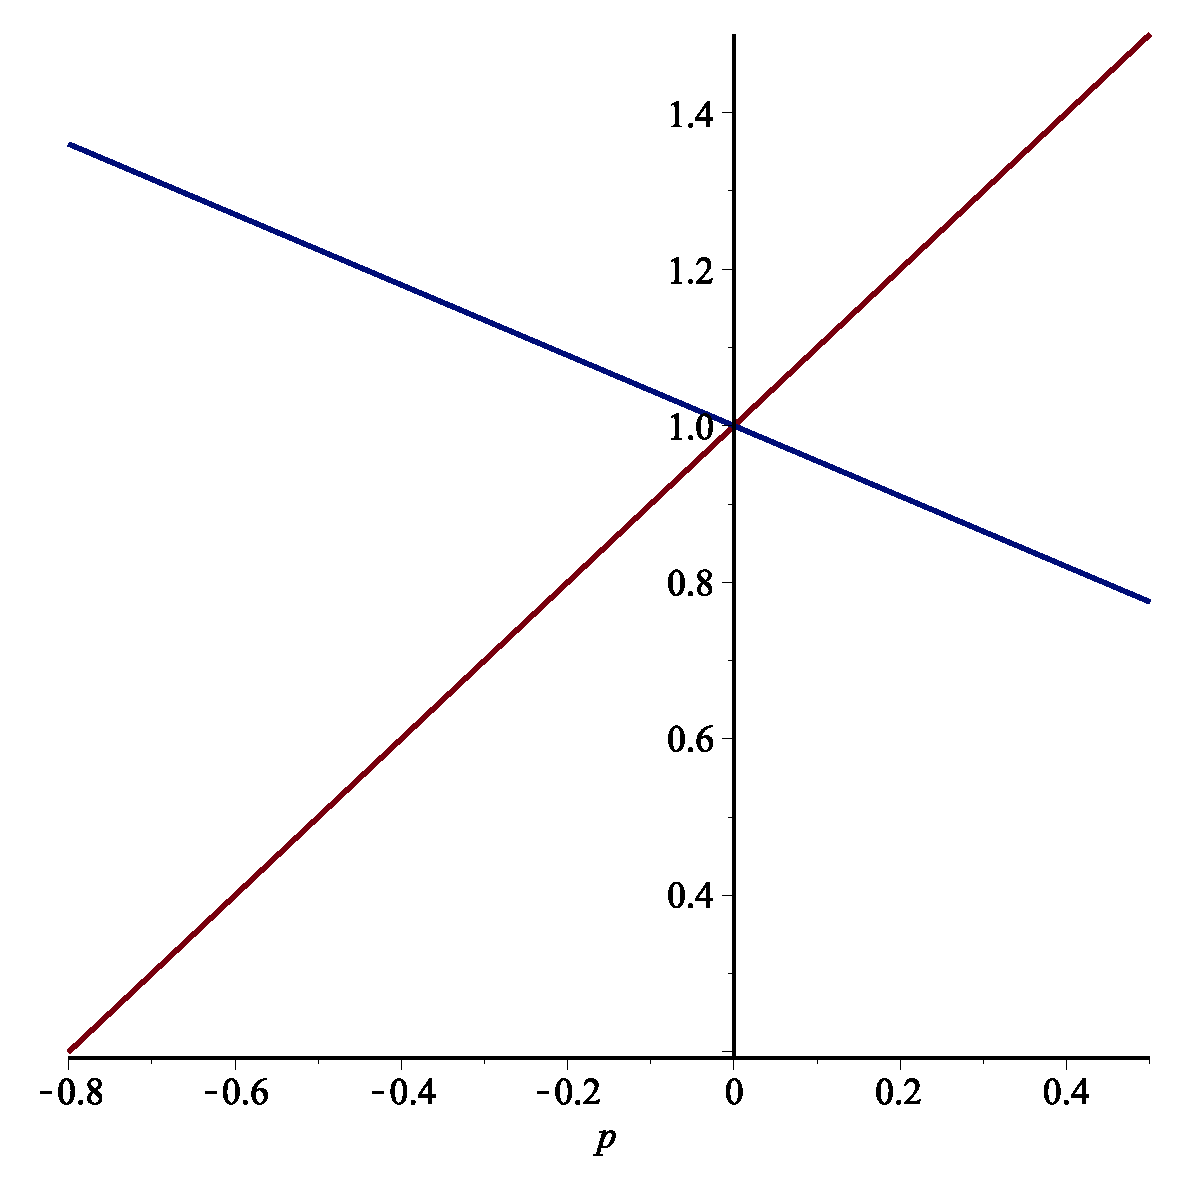
\includegraphics[width=0.60\textwidth]{CurveLinearElasticity}
	\caption{Pure Traction test result for a linear elastic material}
	\label{fig:PureTractionLinearElasticity}
\end{figure}

\section{Pure Traction test for a St Venant Kirchhoff Material}

The elastic energy $W_{SVK}$ for a St Venant Kirchhoff material is the same as  the linear elasticity case but with Green-strain $\epsilon_i=\frac{1}{2}(s_i^2 -1)$ instead of linearized strain.
\subsection{Engineering Pressure}
When solving for the radial extension, we get :
\begin{align*}
\frac{\partial W_{SVK}}{\partial s_2} = \frac{\partial W_{SVK}}{\partial \epsilon_2}\frac{\partial \epsilon_2}{\partial s_2}= 0 \\
V_0 (2\lambda (\epsilon_1+2 \epsilon_2) + 4\mu \epsilon_2)=0 \\
\epsilon_2 = -\nu \epsilon_1
\end{align*}
Thus the 2 deformations are proportional but not the stretch ratio since $s_i=\sqrt{1+2\epsilon_i}$. 

For longitudinal stretch, we get the following relations :
\begin{align*}
\frac{\partial W_{SVK}}{\partial s_1} = \frac{\partial W_{SVK}}{\partial \epsilon_1}\frac{\partial \epsilon_1}{\partial s_1}= 0 \\
E s_1 \epsilon_1=p 
\end{align*}

When plotting the curve $p=s_1 \epsilon_1 =\frac{s_1}{2}((s_1)^2-1)$ we see that the same stress can be produced for several value of stretch. However, for $s_1 > \frac{\sqrt{3}}{3}$ it is possible to get an unique value of stress. This means that the cylinder cannot be compressed more than $s_1=\frac{\sqrt{3}}{3}$ for this material.

\begin{figure}[!htbp]
	\centering
    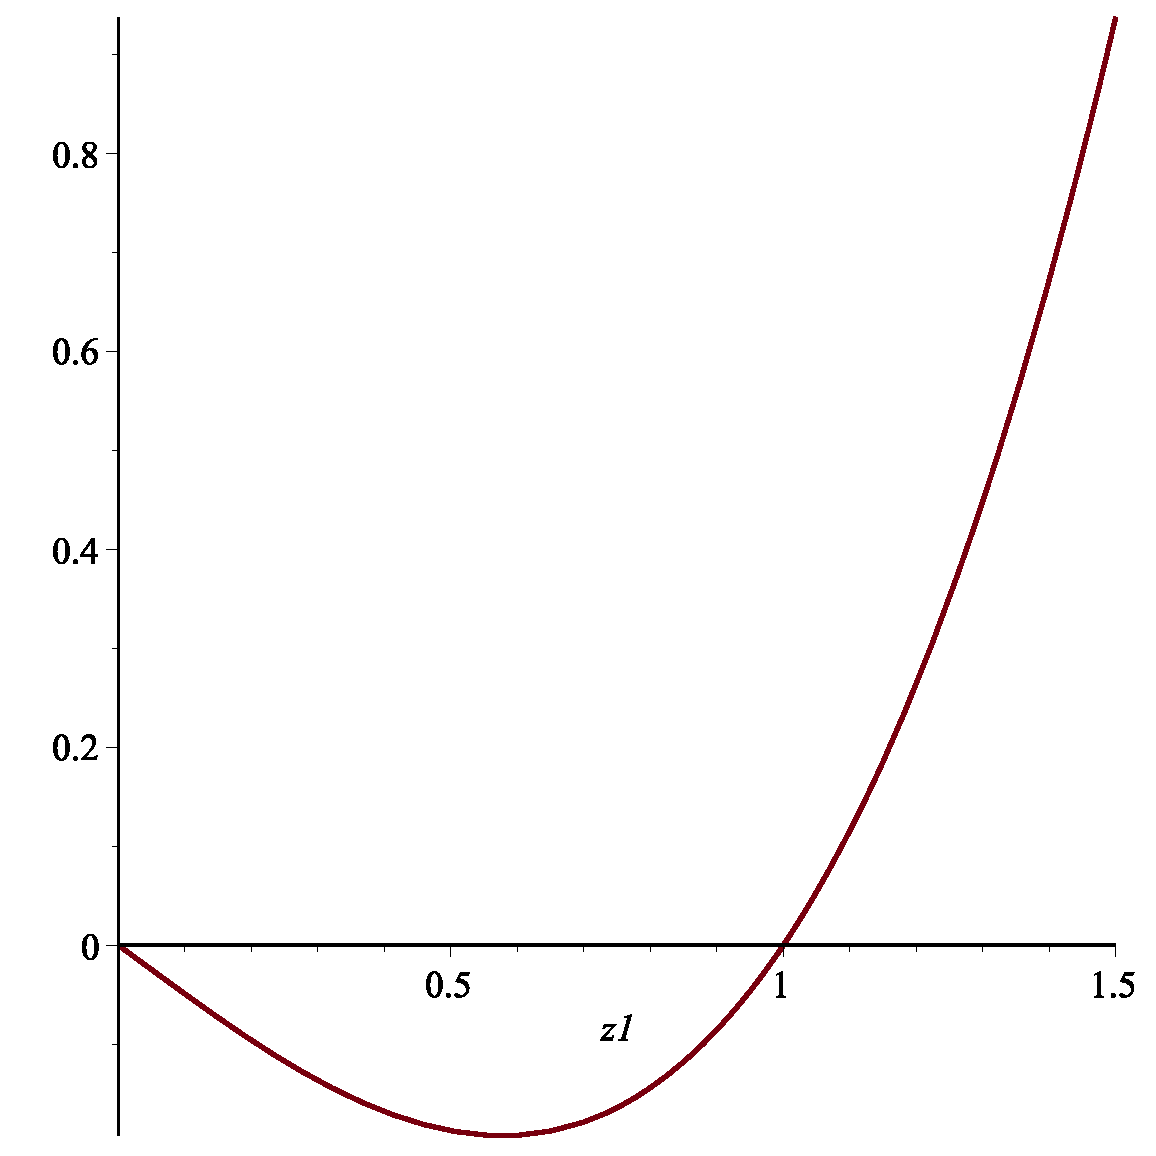
\includegraphics[width=0.60\textwidth]{StressSVK}
	\caption{Longitudinal Stress as a function of longitudinal stretch for a St  Venant Kirchhoff Material. This corresponds to the curve $p=\frac{s_1}{2}((s_1)^2-1)$}
	\label{fig:PureTractionSVKStress}
\end{figure}

For the domain $[\frac{\sqrt{3}}{3},+\infty]$  the 2 stretch ratios are plot as a function of the applied pressure corresponding to the three equations parameterized by $s_1$:
\begin{align*}
p&=\frac{E s_1 }{2}(s_1^2 -1) \\
\epsilon_1&=\frac{1}{2}(s_1^2 -1)\\
\epsilon_2 &= -\nu \epsilon_1
\end{align*}

In the figure below are also plotted the 2 stretch ratios in the case of linear elasticity with the same Young Modulus and Poisson ratio. We can see that for small stretch the 2 materials behave in a similar way. 

\begin{figure}[!htbp]
	\centering
    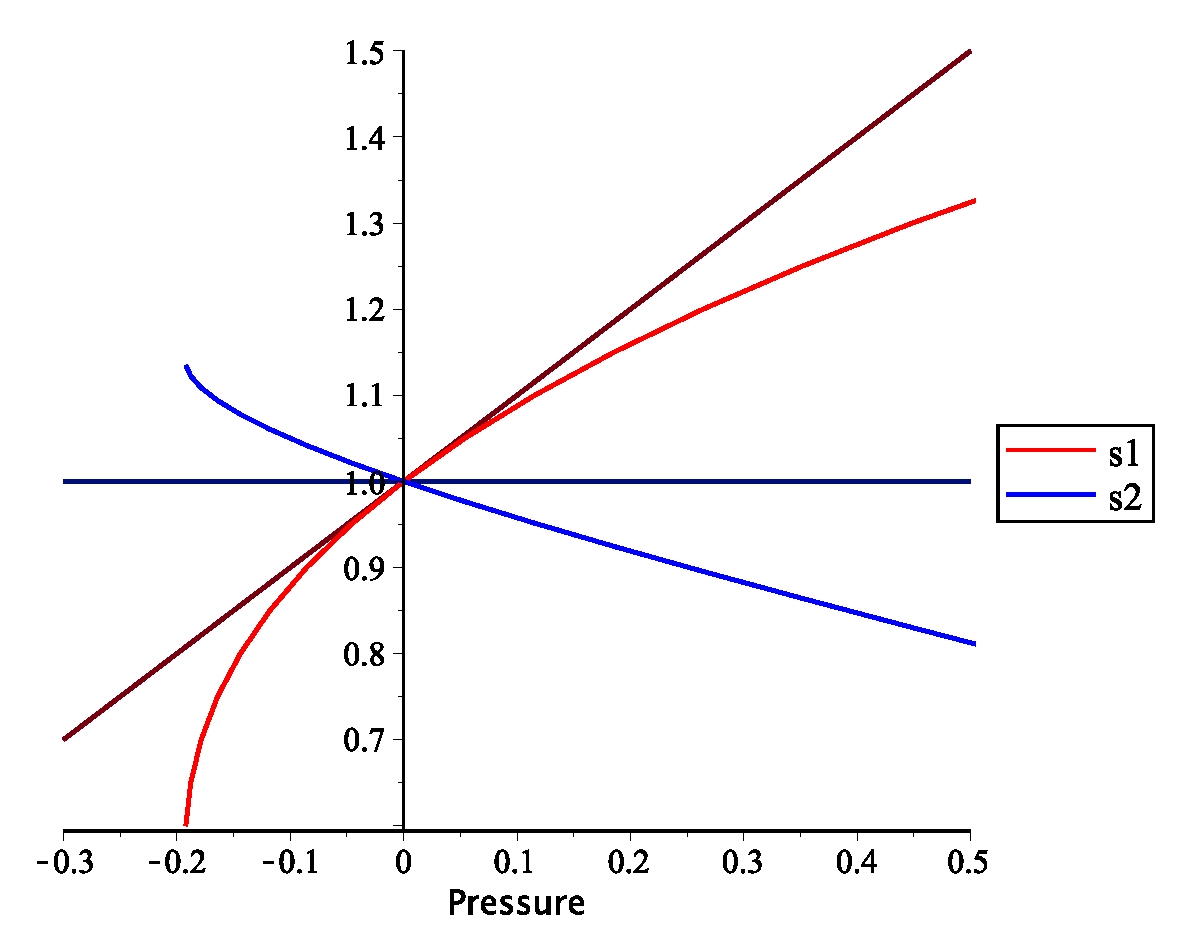
\includegraphics[width=0.60\textwidth]{CurveSVK}
	\caption{Longitudinal and radial stretch as a function of applied pressure for a St  Venant Kirchhoff Material}
	\label{fig:PureTractionSVK}
\end{figure}

\subsection{Real Pressure}

In this case, we still have $\frac{\partial W_{SVK}}{\partial s_2} =0$ and therefore $\epsilon_2 = -\nu \epsilon_1$.
The second derivative now becomes : $\frac{\partial W_{SVK}}{\partial s_1}=(s_2)^2 p$ which translates as 
$\frac{\partial W_{SVK}}{\partial s_1}=s_1 \epsilon_1 E=(s_2)^2 p=(1-2\nu\epsilon_1)p$. 

Therefore we obtain a third order algebraic equation :
\[
E^2 \epsilon_1^2(1+2\epsilon_1)=p^2(1-2\nu\epsilon_1)^2
\]


\section{Pure Traction test for a compressible St Venant Kirchhoff Material}

\subsection{Engineering Pressure}
The elastic energy $W_{CSVK}$ for a compressible St Venant Kirchhoff material is equal to $W_{SVK}$ with an additional term when the material is compressed ($J<1$).
The corrective term is $ \eta |J-1|^3_{-}$ where $\eta=\frac{3}{4}(\lambda+2\mu)$ and $|x|_{-}$ is the negative part of $x$ ($|x|_{-}= -x$ if $x<0$ and $0$ otherwise).
\[
W_{CSVK}=V_0 (\frac{\lambda}{2}  (\epsilon_1+2 \epsilon_2)^2 +\mu ((\epsilon_1)^2+2 (\epsilon_2)^2)) -\eta (s_1 (s_2)^2-1)^3
\]

Writing  $\frac{\partial W_{SVK}}{\partial s_2}=0$ no longer leads to a simple relationship between $\epsilon_1$ and $\epsilon_2$. However, we obtain the following equations :
\begin{align}
&2 s_2 \left (\lambda (\epsilon_1 + 2 \epsilon_2) + 2\mu \epsilon_2 - 3\eta (J-1)^2 s_1 \right )=0 \nonumber \\
& \lambda (\epsilon_1 + 2 \epsilon_2) + 2\mu \epsilon_1 - 3\eta (J-1)^2 \frac{J}{(s_1)^2} = \frac{p}{s_1} \label{eq;csvk-p} \\
& \frac{\lambda}{2} ((s_1)^2-1)  + (\lambda+\mu) (\frac{J}{s_1} -1) - 3\eta (J-1)^2 s_1 =0 \label{eq;csvk}
\end{align}

From equation \ref{eq;csvk}, we see that given a value of $s_1$ such that $0\leq s_1 \leq 1$, we can obtain a value of $J$ by solving a second order equation and taking the positive root of this equation.  Given $J$, we obtain $\epsilon_1=\frac{1}{2}((s_1)^2 -1)$ and $\epsilon_2=\frac{1}{2}(\frac{J}{s_1}-1)$ and the pressure with \ref{eq;csvk-p}. This leads to the following pressure / stretch curve :
\begin{figure}[!htbp]
	\centering
    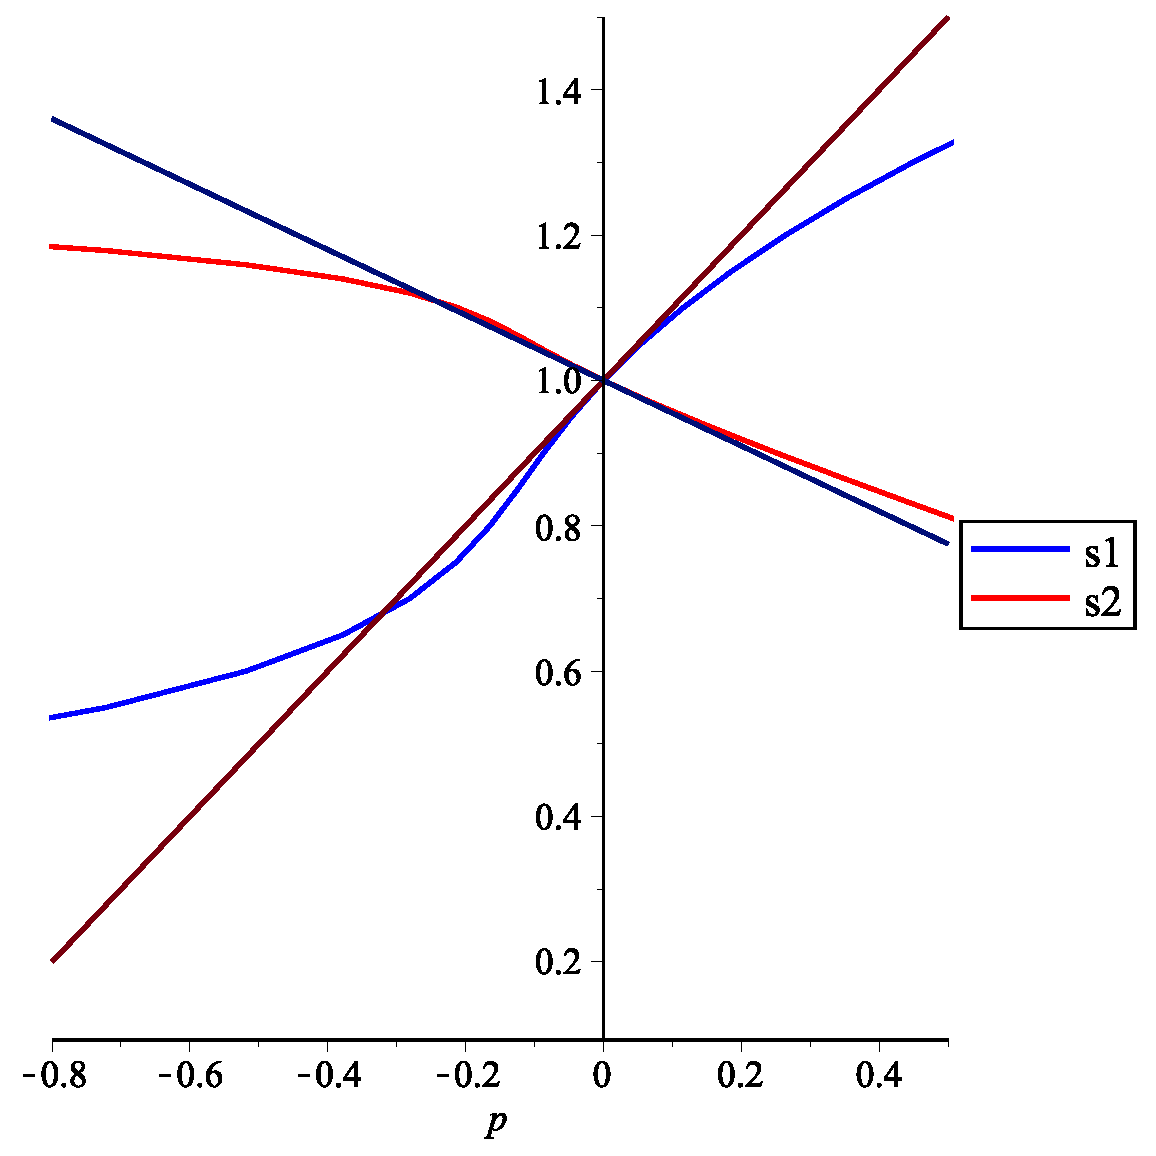
\includegraphics[width=0.60\textwidth]{CurveCSVK}
	\caption{Longitudinal and radial stretch as a function of applied pressure for a compressible St Venant Kirchhoff Material}
	\label{fig:PureTractionCSVK}
\end{figure}
 
\subsection{Real Pressure}

We use the following equation   $\frac{\partial W_{SVK}}{\partial s_1}=(s_2)^2 p$ instead of  $\frac{\partial W_{SVK}}{\partial s_1}=p$.
Thus we have :
\begin{align}
&2 s_2 \left (\lambda (\epsilon_1 + 2 \epsilon_2) + 2\mu \epsilon_2 - 3\eta (J-1)^2 s_1 \right )=0 \nonumber \\
& \lambda (\epsilon_1 + 2 \epsilon_2) + 2\mu \epsilon_1 - 3\eta (J-1)^2 \frac{J}{(s_1)^2} = \frac{p(s_2)^2}{s_1} \label{eq;csvk-newp} \\
& \frac{\lambda}{2} ((s_1)^2-1)  + (\lambda+\mu) (\frac{J}{s_1} -1) - 3\eta (J-1)^2 s_1 =0 
\end{align}
We proceed similarly to the engineering pressure. Set $s_1$ solve in J with the last equation and get the pressure with the modified equation\ref{eq;csvk-newp}.

\section{Pure Traction test for a Neo Hookean Material}


\subsection{Engineering Pressure}
The elastic energy of a Neo-Hookean material $W_{NH}$ is given as :
\[
W_{NH} = V_0 (C_1 (\frac{\Trace (\defGrad^T \defGrad)}{J^{2/3}}-3) + D_1 (J-1)^2)
\]
where $C_1=\mu/2$ and $D_1=\frac{\lambda}{2}+\frac{\mu}{3}$. After replacing $(s_2)^2$ by $J/s_1$, the Pure Traction test energy translates as :
\[
W_{NH} = V_0 \left (C_1 \left (\frac{(s_1)^3 +2 J}{s_1 J^{2/3}}-3\right ) + D_1 \left (J-1\right)^2 \right)
\]
After writing $\frac{\partial W_{NH}}{\partial J}=0$ we obtain the following relation :
\[
D_1 J^{\frac{5}{3}}(J-1) + \frac{C_1}{3} \left (\frac{J}{s_1}-(s_1)^2\right )=0
\]
Thus for a given value of $J$, one has to solve a third order polynomial in $s_1$ which is done in closed form by Maple. By writing $\frac{\partial W_{NH}}{\partial s_1}=p$ one obtains the expression of the pressure as a function of $s_1$ and $J$ which becomes a sole function of $J$. 
 This leads to the   pressure / stretch curve of figure \ref{fig:PureTractionNH}:
\begin{figure}[!htbp]
	\centering
    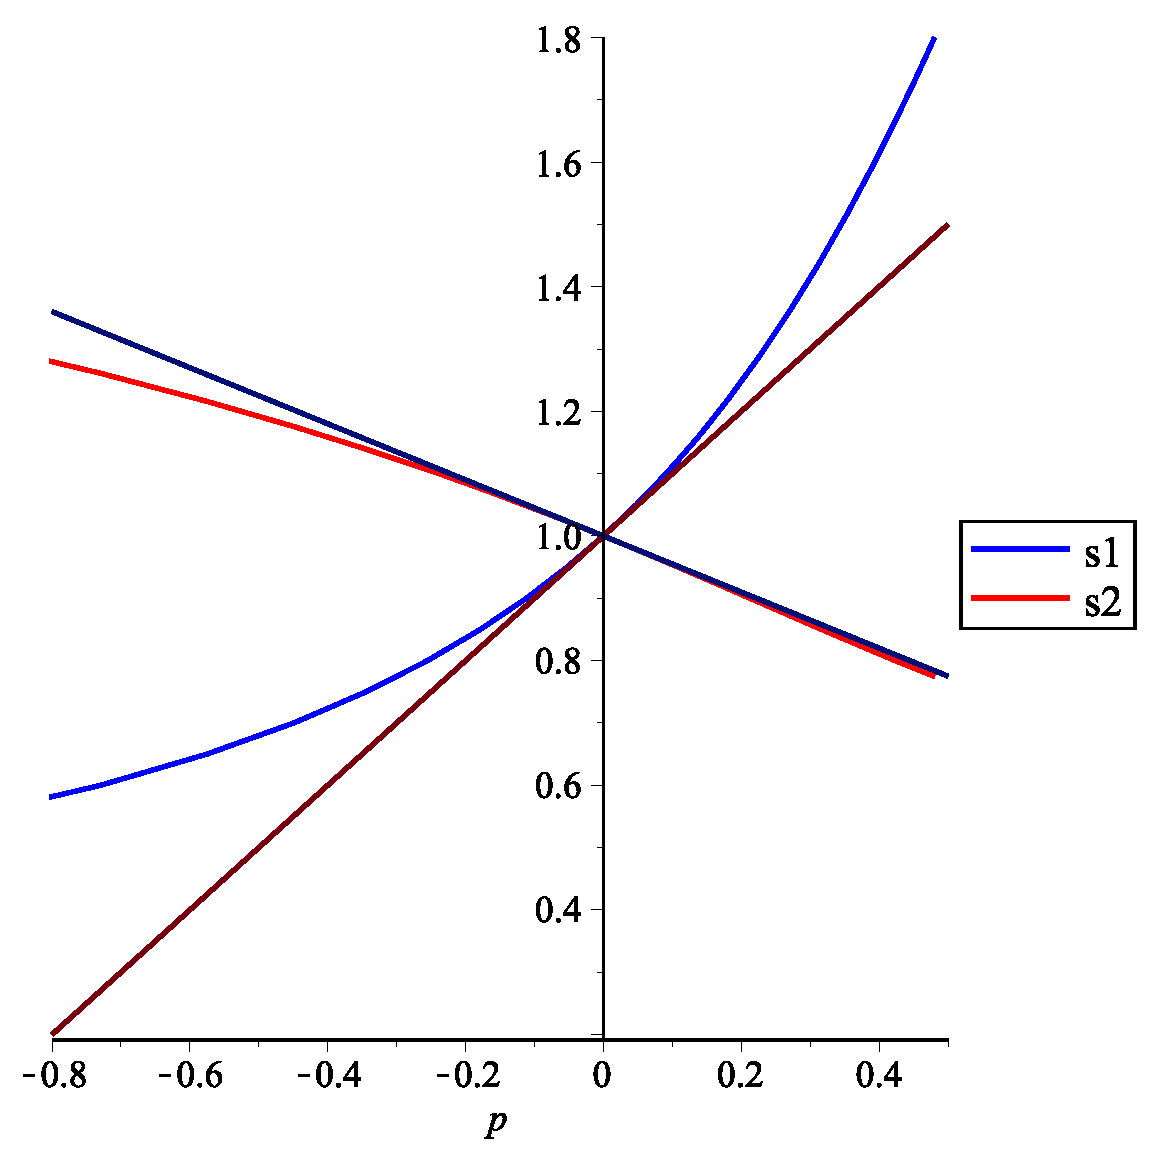
\includegraphics[width=0.60\textwidth]{CurveNH}
	\caption{Longitudinal and radial stretch as a function of applied pressure for a Neo-Hookean Material}
	\label{fig:PureTractionNH}
\end{figure}

\subsection{Real Pressure}
We write the energy as a function of $s_1$ and $s_2$ and then writes 
\[
W_{NH} = V_0 \left (C_1 \left (\frac{(s_1)^2 +2 (s_2)^2}{ (s_1)^{2/3} (s_2)^{4/3}}-3\right ) + D_1 \left (s_1(s_2)^2-1\right)^2 \right)
\]
We can see that deriving with respect to $J$ and setting to 0 is the same as deriving with respect to $(s_2)^2$ and equating to zero.
Therefore we can proceed as in the Engineering presure case but switch $\frac{\partial W_{SVK}}{\partial s_1}=p$. with $\frac{\partial W_{SVK}}{\partial s_1}=(s_2)^2 p$ which is very easy.

\section{Pure Traction test for a Mooney Rivlin Material}

The elastic energy of a Mooney Rivlin  material $W_{NH}$ is given as :
\[
W_{MR} = V_0 \left (C_1 (\frac{\Trace (\rcgd)}{J^{2/3}}-3) + \frac{C_2}{2} (\frac{(\Trace \rcgd)^2 -\Trace (\rcgd^2) }{J^{4/3}}-3) + D_1 (J-1)^2 \right )
\]
where $\rcgd=\defGrad^T \defGrad$, $C_1=C_2=\mu/4$ and $D_1=\frac{\lambda}{2}+\frac{\mu}{3}$. For the Pure Traction test, this translates as :
\[
W_{MR} = V_0 \left (C_1 \left (\frac{(s_1)^2 +2\frac{J}{s_1}}{J^{2/3}}-3\right ) + C_2 \left ( \frac{2 s_1  + \frac{J}{(s_1)^2}}{J^{1/3}}-3\right )+ D_1 \left (J-1\right)^2 \right)
\]
Solving $\frac{\partial W_{SVK}}{\partial J}=0$ leads to an expression of $J$ as a function of $s_1$ which in terms leads to a expression of type $f(s_1)=p$ in Maple. This leads to the   pressure / stretch curve of figure \ref{fig:PureTractionMR}:
\begin{figure}[!htbp]
	\centering
    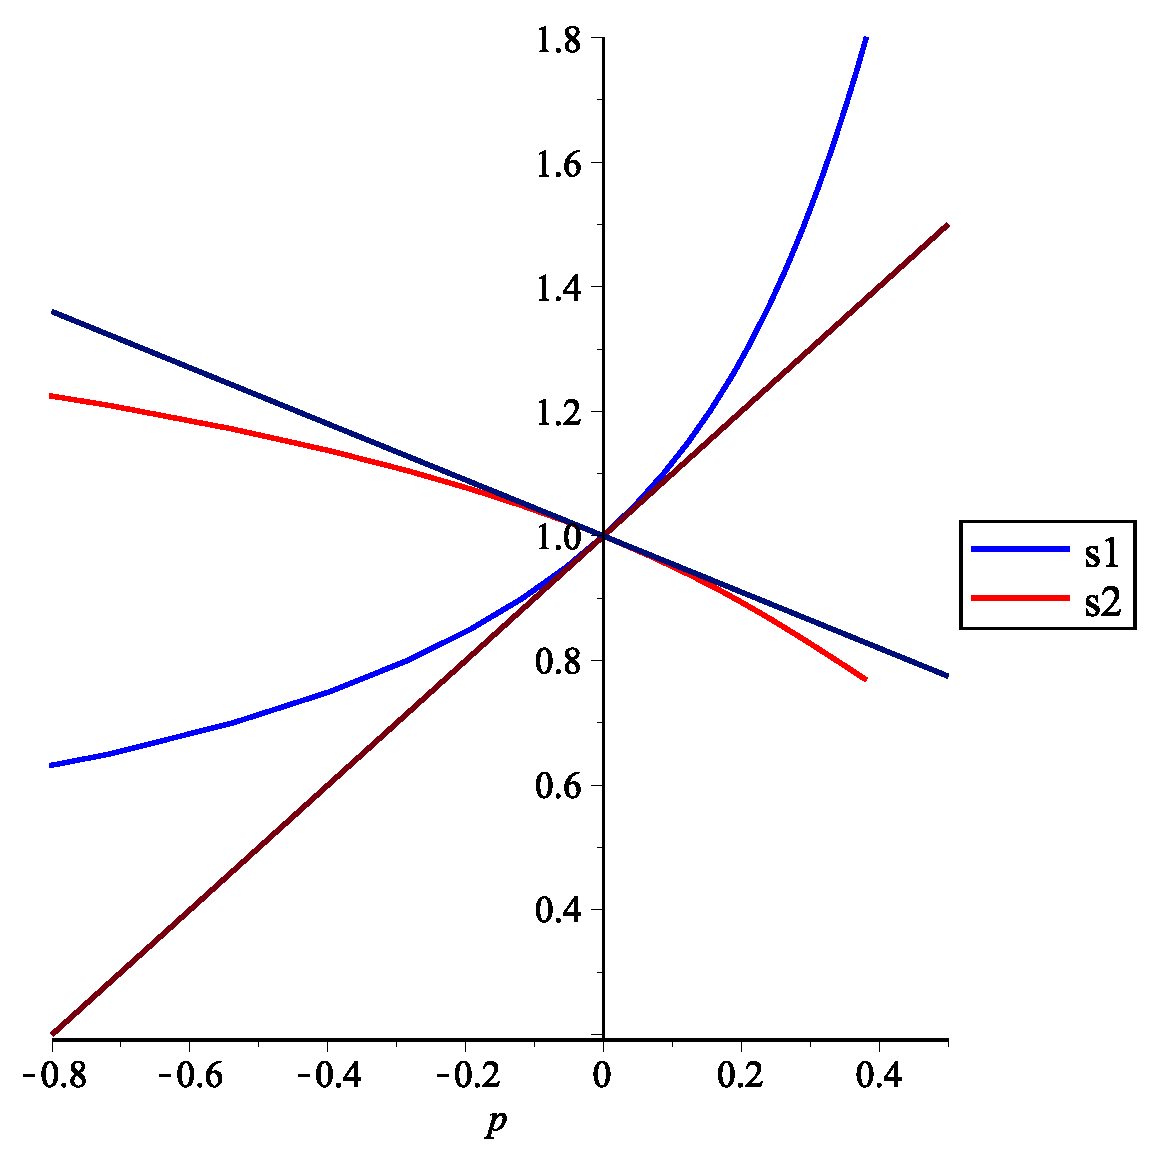
\includegraphics[width=0.60\textwidth]{CurveMR}
	\caption{Longitudinal and radial stretch as a function of applied pressure for a Mooney-Rivlin  Material}
	\label{fig:PureTractionMR}
\end{figure}

The same applies here for real pressure. Only replace $f(s_1)=p$ with $\frac{s_1 f(s_1)}{J}=p$

\end{document}          

